\documentclass[a4paper,11pt,twoside,openright]{scrbook}

\usepackage{swThesis}
\usepackage{amsmath}
\usepackage[htt]{hyphenat}
\usepackage{lipsum}
\usepackage{standalone}
\standalonetrue

\bibliography{bibliography}

% Figures
\graphicspath{./figs}

\begin{document}

\chapter{Cheminformatics and high-content imaging} \label{chapter:cheminformatics}

\section{Introduction}

\subsection{Cheminformatics}
% Introduction to cheminformatics
The term ``cheminformatics'' was first coined in 1998\cite{Brown1998} although the use of computers to interact with chemical data predates this by many years, with early systems used to index, search and catalogue databases of chemical compounds. \cite{Ray1957}
Most of the early work in this field was concerned with efficient means to search large chemical databases for similar molecules or molecules containing certain sub-structures.
This early work developed a number of important methods to generate, represent and compare chemical structures in a time of limited computational power, as a by-product these methods are very efficient and are still used today as the size of chemical databases has grown alongside computational power.

It was later on that researchers attempted to correlate biological activity with physiochemical parameters and give rise to structure activity relationships (SAR), this was partly due to the advancement of statistical techniques which gave rise to new tools such as multiple linear regression.
One of the first quantitative SAR (QSAR) studies was carried out by Hansch and Fujita, in which they found the lipophilicity of a molecule correlated strongly with biological activity \cite{HanschCitation}.
Since then the QSAR field has advanced to include many more parameters and in now a key part in most empirical drug discovery efforts.

% cheminformatics for drug library design
% chemical space and all that
Another use of cheminformatics in drug discovery is the analysis and design of compound screening libraries.
% mention lipinski's RO5 as an established method to filer compound collections?
In industrial high-throughput screening a full-deck compound library typically contains several million small molecules.
Screening this entire library is a costly endevour, even for pharmaceutical companies, and therefore a lot of research has been carried out in how to maximise the value and information gained from screening these large compound collections.
One of the ways compound libraries can be optimised is by covering a large a range of chemical space as possible.
A compound library that contains many extremely similar molecules may be useful in certain specific circumstances, but in most cases this is viewed as a redundancy and a library which covering the same chemical space with fewer compounds would reduce costs.
Alternatively, a compound collection of equal size which contains more diverse chemistry may lead to a more varied selection of lead candidates. \cite{Clemons2011}
The concept of chemical space in compound collections can also be used to identify potential blind-spots or bias in drug discovery libraries, which are areas of chemical space with potential biological potential that are not covered by an existing library, in contrast to areas of chemical space which are well covered by a compound collection but have historically failed to show biological activity, termed ``dark chemical matter''. \cite{Wassermann2015}


\subsection{Structure activity relationships}
% structure activity relationship
% how this is used in target-based drug discovery
 % lead optimisation for affinity and specificity
% but how is this used in a target-agnostic setting?
    % any examples?
A structure activity relationship is the link between a chemical's structure and its effect in a biological system, which underpins much of the medicinal chemistry field.
The underlying premise of SAR is that compounds with similar structures and physiochemical properties have similar biological effects by virtue of binding to the same or similar targets.
This idea is commonly applied during lead optimisation whereby a candidate molecule is iteratively modified in order to optimise parameters such as specificity and affinity, all the while ensuring that these modifications do not disrupt binding to the desired target, leading to the identification and determination of functional groups which are required for target engagement and biological activity.

% multiparametric
Relating changes to a compound's structure to biological activity is relatively straightforward if compound activity can be represented as a single variable such as binding affinity or EC$_{50}$, applying quantitative SAR (QSAR) to multiparametric data such as that found with high-content imaging is not as well defined.




\subsection{Chemical similarity}
Despite the premise of QSAR as ``\textsl{similar molecules} have similar biological effects'' there is the challenge of how to measure similarity between chemical structures.
Chemical structures can be represented in a number of different formats and we typically think of the skeletal 2D graphical representation (figure \ref{figure:mol_encodings} A) when considering complex organic molecules which have to be interpreted by chemists.
Computers however require a different format to efficiently store and parse chemical structure data.
SMILEs (simplified molecular input line entry system) and InChIs (international chemical identifier) are two formats which encode chemical structures as short character strings representing atoms as human readable characters (such as \texttt{CH} for carbon and hydrogen) with other symbols to represent branches and sterochemistry etc (figure \ref{figure:mol_encodings} B\&C).
These relatively simple formats sometimes suffer from ambiguity, in which a single encoding could represent several molecules, or a single molecule could be
represented by multiple valid encodings.
A less ambiguous but also less human-readable file format is SDF (structure data file) or Molfile, which encode chemical structures as a table of x, y, z co-ordinates and bonds for each atom (figure \ref{figure:mol_encodings} D).

\begin{figure}
    \fcapsideright{
    \caption[Different methods to encode chemical structure]{
Different methods to encode the chemical structure of a molecule (aspirin).
\textbf{(A)} A 2D skeletal graphical representation commonly used by chemists.
\textbf{(B)} SMILE format, a concise relatively human readable format encoding atoms as characters.
\textbf{(C)} InChI format, another commonly used string format which is less human readable but contains more details to reduce ambiguity.
\textbf{(D)} SDF / Mol format. A tabular format which lists the co-ordinates of atoms in 3 dimensions along with bonds and distances.
}
} {
    \includegraphics[scale=1.5]{ch5molEncodings}
    \label{figure:mol_encodings}
}
\end{figure}

% chemical similarity
    % required properties of a chemical fingerprints
    % daylight fingerprints + tanimoto distances
    % ECPF? USRCAT
Given these encodings of chemical structure and the task to calculate similarity (or distance) between molecules, the most direct and simple method is to calculate distance based on the string encodings (usually SMILE format), such as hamming distance or longest-common-substring divided by total length between two SMILE strings.\cite{Ozturk2016}
However, these naive methods  suffer from a number of drawbacks, mainly stemming from the ambiquity and variability of SMILE encodings which limit their widespread use. \cite{citation_needed}
A more nuanced approach to measuring chemical similarity is to first calculate  compound fingerprints such as daylight or extended connectivity fingerprints (ECFP) \cite{citation} which are abstract representations of molecules in the form of fixed-length binary arrays -- generated from local patterns in the molecule such as the identity of neighbouring atoms (where neighbouring is extended to several bonds away).
The distance between compound fingerprints can then be found using one of a variety of distance metrics.
To compare the binary compound fingerprints the most commonly used metric is Tanimoto similarity ($T_s$) and distance\footnote{Whilst not a distance in the  strict mathematical sense it is commonly referred to as a distance metric.} ($T_d$), where $T_s$ is defined as the ratio of common elements between two equal length fingerprints divided by the length of either fingerprint, and $T_d = -\log_2(T_s)$.
Another approach to molecular fingerprinting is to summarise the 3D shape of a molecule.
Ultrafast shape recognition (USR) was developed and used for \textit{in silico} drug screening to efficiently describe molecular shape in 12 measurements.
USR however was optimised for computational efficiency at the expense of detailed information and is agnostic to the atom types contained in the molecule.
This drawback led to an extension of USR (USRCAT - USR with CREDO atom types) which was later developed for users to search the protein data bank and describes a molecule's 3D shape and constituent atoms. \cite{Schreyer2012}
Recently a number of studies have leveraged advances in the machine learning field to generate alternative chemical fingerprints using neural networks. \cite{Kearnes2016a,Feinberg2018,Ma2018,Liu2018}
The idea behind these methods is that deep neural networks are able to learn appropriate representations of the input data in order to maximise performance in a certain task.
They typically represent chemical structures as un-directional graphs of atoms, and apply convolutional techniques -- which have proven themselves in image-related tasks -- to the graph structures to generate molecular fingerprints which can be used in downstream machine learning and cheminformatics work.


\subsection{Application of cheminformatics to high-content screening}
Much of the work in cheminformatics is carried out in industrial rather than academic laboratories, coupled with the relatively immature field of high-content imaging means has resulted in a sparsity of published research in the application of cheminformatics to high-content imaging and screening.

% Young et al paper summary
One of the earliest papers which combined cheminformatics with image-based screening was by Young \textit{et al.}\cite{Young2008} who screened a library of 6,547 compounds in HeLa cells and extracted 30 morphological features regarding nuclei morphology.
They used factor analysis and hierarchical clustering to group their compound library into 7 clusters describing similar nuclear morphologies, and created matrices of phenotypic similarity with consine similarity of phenotypic features and compound similarities with Tanimoto coefficients of ECFP features.
They then found a correlation between the rank ordering of phenotypic similarities and compound similarities, as well as identified instances of ``activity-cliffs'' when two structurally similar compounds demonstrated very different phenotypic activities which matched up to known SAR studies on the two compounds.

% Wawer compound library design summary
A second study by Wawer \textit{et al.}\cite{Wawer2014b} incorportated high-content morphological profiling to construct compound libraries based on the diversity of biological response as opposed to diversity of chemical space.
Using a library of 31,000 compounds, they performed a image-based morphological screen and selected a subset of compounds which produced a diverse range of bioactivities.
They then compared this subset to a second subset generated by maximising diversity of chemical space, and investigated the performance of each subset of compounds in a wide range of previously performed cell-based screens.
They found that subsetting compounds based on morphological diversity resulted in an increased performance compared to compounds chosen on chemical diversity or compounds chosen at random.

Another paper published by the same group\cite{Wawer2014c} developed a method for SAR with high-dimensional profiling data, assessing both high-content imaging and gene expression profiling datasets.
They used pattern mining techniques originally developed in advertising and marketing to find frequently linked sub-structures with certain biological activities.

% find which papers have been published and v. briefly summarise them
% Young Bender, Clemons Wagner
% activity cliffs
    % representing a continuous landscape of chemical similarity and biological
        % activity
    % real biology or artefacts of molecular representation?


\subsection{Aim of this chapter}
This chapter is based on work using the BioAscent compound library which is supplied with detailed structural information of each of the 12,000 compounds.
My aim was to incorporate this chemical information with existing public datasets and my own high-content imaging data in a way to aid target convolution as well as investigate the link between chemical structure structure activity relationship (SAR) applied to cellular morphology as an indicator of compound activity.




%%%%%%%%%%%%%%%%%%%%%%%%%%%%%%%%%%%%%%%%%%%%%%%%%%%%%%%%%%%%%%%%%%%%%%%%%%%%%%%%
%%%%%%%%%%%%%%%%%%%%%%%%%%%%%%%%%%%%%%%%%%%%%%%%%%%%%%%%%%%%%%%%%%%%%%%%%%%%%%%%
%%%%%%%%%%%%%%%%%%%%%%%%%%%%%%%%%%%%%%%%%%%%%%%%%%%%%%%%%%%%%%%%%%%%%%%%%%%%%%%%




\section{Results}


% compare MOA prediction from phenotypic data with the predicted target obtained
% from chemical similarity matches to public databases (ChEMBL)

% evaluation of how chemical similarity matches phenotypic similarity within the
% BioAscent dataset

\subsection{The BioAscent library contains clusters of phenotypically similar compounds}

In order to compare the phenotypic profiles produced by compounds in the BioAscent library, active compounds were selected based on on the L$_1$ norm distance from the negative control centroid (figure (\ref{figure:compound_activity})).
As many of the compounds were cytotoxic and produced images containing only a few dying cells which do not produce robust morphological measurements, an activity window was used to exclude cytoxic compounds.


\begin{figure}
    \captionsetup{width=0.8\textwidth}
    \caption[Selecting active compounds based on distance]{
Selection of active BioAscent compounds based on the L$_1$ norm distance from the DMSO negative control centroid in PCA space.
Lower and upper bounds of the selected compounds are indicated by dashed lines. In total 1244 compounds were selected.}
    \includegraphics[width=0.6\textwidth]{ch5compoundActivities}
    \label{figure:compound_activity}
\end{figure}

Hierarchical clustering of morphological profiles produced by these phenotypically active compounds showed that despite the chemical diversity of the BioAscent library, the active compounds formed distinct clusters of compounds which produced similar cellular morphologies (figure \ref{figure:morph_cluster} A).
To confirm the validity of the clustering, the hierarchical labels were compared with clusters found in an unsupervised algorithm.
The morphological profiles were embedded into lower dimensional space using the t-SNE algorithm \cite{Maaten2008} which aims to preserve local structure within the data and reveals clusters of similar points in an unsupervised approach.
When these points were coloured by the cluster labels idenfified by hierarchical clustering they appeared to match up with the tSNE embedding (figure \ref{figure:morph_cluster} B).

\begin{figure}
    \captionsetup{width=0.8\textwidth}
    \caption[Morphological clustering of the BioAscent library]{
Morphological clustering of active compounds within the BioAscent library.
    \textbf{(A)} Hierarchical clustering of the 1244 active BioAscent compounds based on a distance matrix of principal components.
    Clusters formed by cutting the produced dendrogram.
    \textbf{(B)} Unsupervised t-SNE clustering of active BioAscent compounds based on principal components of morphological features.
    Points are labels derived from the hierarchical clustering.
}
    \includegraphics[width=0.9\textwidth]{ch5phenotypicClustersBoth}
    \label{figure:morph_cluster}
\end{figure}
% maybe add some images of example morphologies produced by each cluster



\subsection{The BioAscent library is chemically diverse}
The BioAscent library is marketed as chemically diverse, yet I still wanted see to what degree this is true, and if there are clusters of chemically similar compounds such as those based around a common scaffold.
All 13,000 BioAscent compounds were converted into molecular fingerprints to produce a distance matrix between all pairs of compound fingerprints, this was then clustered using agglomative hierarchical clustering.
As could be predicted, the heatmaps and dendrograms did not reveal any large clusters of structurally similar compounds in the 13,000 compound library.
This chemical diversity continued when the compounds were filtered to only contain the phenotypically active molecules.
The use of more novel compound fingerprinting techniques such as USRCAT \cite{Schreyer2012} and autoencoded features \cite{Gomez-Bombarelli2016} did not increase the degree of clustering.

%TODO insert figure of (lack of) compound similarity clustering for both 13K and
%active

Rather than looking at large-scale clustering of many thousands of compounds with hierarchical clustering, I tried the Butina clustering method to identify small collections of structurally similar compounds.
This method does not return similarity measures, but rather groups compounds into bins of similar compounds \cite{Butina1999}.
After removing clusters which contained fewer than 3 compounds, this left 96 clusters, with the largest cluster containing 20 compounds and 58\% of the clusters containing only 3 compounds (figure \ref{figure:butina_clusters}).

\begin{figure}
    \captionsetup{width=0.8\textwidth}
    \caption[Histogram of structural cluster sizes and example of molecules within a cluster]{
        \textbf{(A)} Histogram of number of compounds within structurally similar clusters, with most clusters only containing 3 molecules.
        \textbf{(B)} An example of one of the structurally similar clusters as found with the Butina clustering algorithm. 
}
    \includegraphics[width=0.5\textwidth]{ch5butinaClusterBoth}
    \label{figure:butina_clusters}
\end{figure}



\subsection{There is little evidence that structurally similar molecules produce similar cellular morphologies}

Following the premise of SAR, structurally similar molecules are likely to share the same protein binding site, therefore activiting the same or similar signalling pathways and producing similar cellular morphologies.
I investigated to what extend structurally similar molecules in the BioAscent library produce similar cellular morphologies, and also how structurally similar are compounds which were shown to produce similar phenotypes.
Using the phenotypic clusters as defined in fig.\ref{figure:morph_cluster}, I compared the structural similarity between compounds within these phenotypic clusters compared to a null distribution of compounds picked at random.
I found that compounds within phenotypic clusters were very slightly more structurally similar than compounds picked at random (figure \ref{figure:compound_pheno_corr} A, $p=1.81\times10^{-15}$, $D=0.011$, 2-sample Kolmogorov-Smirnov test).
In addition, I approach the problem from the opposite direction and investigated the phenotypic similarity within clusters of structurally similar molecules as found with the Butina clustering algorithm, compared to the phenotypic similarity between compounds picked at random from the pooled compound list of those contained within Butina clusters.
I again found that structurally similar molecules are more likely to produce similar cellular morphologies than compounds picked at random (figure \ref{figure:compound_pheno_corr} B, $p=0.037$, $D=0.018$, 2-sample Kolmogorov-Smirnov test).

Another approach is two see how well the distance matrix of phenotypic profiles correlates with the distance matrix of chemical structures.
Using Mantel's test of correlation between two distance matrices \cite{Mantel1967}, I found no significant correlation between the phenotypic and structural distance matrices for the active 1244 compound subset ($r = 0.02$, $p = 0.116$).


\begin{figure}
    \captionsetup{width=0.8\textwidth}
    \caption[Comparison of structural and phenotypically similar compounds]{
        \textbf{(A)} Tanimoto distance between compounds from within phenotypic clusters (as found in fig. \ref{figure:morph_cluster}) and between randomly paired active compounds.
        ($p=1.81\times10^{-15}$, $D=0.011$, 2-sample Kolmogorov-Smirnov test)
    \textbf{(B)} Phenotypic distance between compounds from within structurally similar clusters and between randomly paired phenotypic profiles.
    ($p=0.037$, $D=0.018$, 2-sample Kolmogorov-Smirnov test)
}
    \includegraphics[width=1.0\textwidth]{ch5compoundSimilarity}
    \label{figure:compound_pheno_corr}
\end{figure}





\subsection{Identifying the putative MoA of phenotypic hits with ChEMBL structure queries}

Another way to utilise the chemical structure data availble with the BioAscent library is through querying publically available databases such as ChEMBL for exact compounds matches or structurally similar compounds.
This returns large amounts of data from a variety of assays in which the compound or a structural analogue was screened against such as targets, EC/IC$_{50}$ values, binding affinities etc.
I set about to see if this historical data could be used to suggest putative MoAs of hits from target agnostic phenotypic screening assays.

For this I used the compounds within 10 phenotypic clusters (figure \ref{figure:morph_cluster}), and for each cluster queried ChEMBL based on a structure similarity search to identify records for either the query compound, or structural analogues.
Then using these compounds identifying which human proteins they have been screened against, and filtering these protein based on EC/IC$_{50}$ values.
This returns a list of Uniprot accession codes which were used with interpro \cite{Finn2017} to test for enrichment compared to a background for each cluster.

Eight out of the ten phenotypic clusters returned at least one significantly enriched target with fold-enrichment ranging between 1.5 and 10.
The most significantly enriched target in 6/8 of the clusters was related to protein kinases, whereas the remaining two were rhodopsin-like GPCRS and adrenergic receptors.

\begin{figure}
    \captionsetup{width=0.8\textwidth}
    \caption[Interpro target enrichment]{
        Enriched interpro targets associated with compounds within one phenotypic cluster.
}
    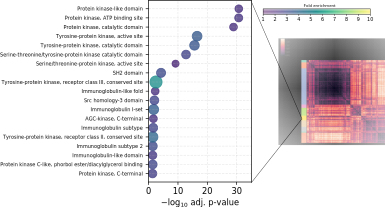
\includegraphics[width=0.8\textwidth]{ch5interpro.png}
    \label{figure:interpro}
\end{figure}



\subsection{Finding phenotypic hits in ``dark chemical space''}

An area of interest in drug discovery is finding new pharmacologically active compounds which occupy new areas of chemical space. \cite{Wassermann2015}
One way to incoporate the phenotypically active hits from the BioAscent library is to query historical screening databases by structural similarity.
To do this I took the list of 1244 phenotypically active BioAscent compounds and performed a structural similarity search on the ChEMBL database to look for those BioAscent compounds which have a large Tanimoto distance from all compounds deposited in the database.

From the 1244 active BioAscent compounds 59 (4.7\%) were found to have no structurally similar analogues in the ChEMBL database (figure \ref{figure:dark_mols}).
To assess if these 59 compounds contained undersireable physiochemical properties which would limit their inclusion in screening libraries explain their absence from historic screening databases I used a quantitative estimate of drug-likeness (QED), \cite{Bickerton2012} to compare the 59 compounds from `dark chemical space' to the 1244 active BioAscent compounds.
The QED metric did not reveal any significant differences in desirable physiochemical properties (QED$_{\text{dark compounds}} = 0.57$,  QED$_{\text{all active}} = 0.60$, 2 sample t-test $t=0.85$, $p=0.39$).


\begin{figure}
    \captionsetup{width=1.0\textwidth}
    \caption[BioAscent hits from dark chemical space]{
BioAscent hits from dark chemical space.
59 phenotypically active BioAscent compounds which had no structurally similar compounds listed in the ChEMBL database as measured.
}
    \includegraphics[width=1.0\textwidth]{ch5darkmols}
    \label{figure:dark_mols}
\end{figure}

%TODO? map all compounds in 2D space, highlighting the dark mols, see if they
%cluster somewhere or are mixed in with all the rest


%%%%%%%%%%%%%%%%%%%%%%%%%%%%%%%%%%%%%%%%%%%%%%%%%%%%%%%%%%%%%%%%%%%%%%%%%%%%%%%%
%%%%%%%%%%%%%%%%%%%%%%%%%%%%%%%%%%%%%%%%%%%%%%%%%%%%%%%%%%%%%%%%%%%%%%%%%%%%%%%%
%%%%%%%%%%%%%%%%%%%%%%%%%%%%%%%%%%%%%%%%%%%%%%%%%%%%%%%%%%%%%%%%%%%%%%%%%%%%%%%%




\section{Discussion and Conclusions}
TODO
% describe what I've achieved
% what I failed to achieve ..?
% chemical similarity is difficult
% would have been a lot easier if I didn't use a chemical diversity library
% rapidly evolving field
% activity cliffs - binding properties change despite very similar structures
% bind to different targets within the same pathway - similar phenotype but can
% be very different structures






%%%%%%%%%%%%%%%%%%%%%%%%%%%%%%%%%%%%%%%%%%%%%%%%%%%%%%%%%%%%%%%%%%%%%%%%%%%%%%%%
%%%%%%%%%%%%%%%%%%%%%%%%%%%%%%%%%%%%%%%%%%%%%%%%%%%%%%%%%%%%%%%%%%%%%%%%%%%%%%%%
%%%%%%%%%%%%%%%%%%%%%%%%%%%%%%%%%%%%%%%%%%%%%%%%%%%%%%%%%%%%%%%%%%%%%%%%%%%%%%%%



\section{Methods}

\subsection{Chemical similarity}
Compound structural information was in the form of .sdf files provided by BioAscent.
To create daylight-like compound fingerprints the RDKit library was used to convert .sdf entries into an RDKit's implementation of the daylight fingerprint using the `rdkit.Chem.Fingerprints.FingerprintMols' function with default parameters.

USRCAT features were generously calculated and supplied by Dr. Steven Shave (Edinburgh).

Latent representations of chemical structure features were calculated using a molecular autoencoder pre-trained on the ChEMBL22 dataset \footnote{www.github.com/cxhernandez/molencoder}, based on the work published by Gomez-Bombarelli \textit{et al.} \cite{Gomez-Bombarelli2016} using one-hot encoded SMILE strings of the molecules.

To compute the distance between RDKit daylight fingerprints the Tanimoto/Jaccard distance was used, in the case of USRCAT and autoencoded features I used the Euclidean distance.
Hierarchical clustering was performed on the distance matrix using the complete linkage method and euclidean distance.
To define clusters from the calculated dendrogram, a threshold was defined as 70\% of the maximum linkage distance which produced 10 clusters.
Butina clustering was implemented using RDKit with Tanimoto distances calculated from daylight fingerprints, with a cutoff value of 0.2.

Mantel's test for comparing two distance matrices was implemented with scikit-bio's implementation using Pearson's correlation coefficient and 999 permutations for testing significance.
The distance matrices used were standardised Euclidean distance for the morphological profiles and standardised Tanimoto distances of the daylight fingerprints for compound structure profiles.


\subsection{BioAscent library screen}

\subsubsection{Compound activity window}
Data was normalised to plate-based controls and features standardised, then transformed with PCA to the minimum number of principal components which accounted for 80\% of the variance in the data.
L$_1$ norm distances were calculated from the DMSO negative control centroid in PCA space.
The lower bound of the activity window was defined visually using a plot of ranked L$_1$ distances.
The upper bound was chosen based on images containing at least 10 cells and visual assessment of images produced by higher L$_1$ distances ensuring images did not consist entirely of dying cell (small, rounded and bright cytoplasmic staining).


\subsection{Phenotypic similarity}
Clustering of morphological profiles was carried out by first calculating a correlation matrix between between all pairs of active compound morphologies.
Hierarchical clustering was performed on the correlation matrix using the complete linkage method and euclidean distance.
To define clusters from the calculated dendrogram, a threshold was defined as 70\% of the maximum linkage distance which produced 10 clusters (figure \ref{figure:dendrogram_cut})

\begin{figure}
    \captionsetup{width=0.8\textwidth}
    \caption[Dendrogram threshold to determine clusters]{
Dendrogram thresholding to determine the number of phenotypic clusters in the active BioAscent compounds.
Dashed line indicates cutoff of 70\% of the maximum linkage distance, resulting in 10 clusters.
}
    \includegraphics[width=0.8\textwidth]{ch5dendrogram}
    \label{figure:dendrogram_cut}
\end{figure}

t-SNE clustering was performed using sklearn's `manifold.TSNE` implementation using the Barnes-Hut approximation with the default parameters.

\subsection{ChEMBL structure searches}
To query the ChEMBL database I used the ChEMBL webresource client \footnote{www.github.com/chembl/chembl\_webresource\_client}.
In order to identify records for similar compounds I first queried structures based on SMILE strings of the BioAscent compounds with a filter to return only compounds with a Tanimoto distance less than 0.1, recording the similar compounds as ChEMBL identifiers.
Then in a second query using the ChEMBL identifiers, I searched for historical screening results against human protein targets and returned a list in the form of Uniprot accession codes.
As this returned a list of all protein targets which had been screened against, I filtered this list to protein targets with an assay EC/IC$_{50}$ value less than 1 $\mu$M.
This was repeated for each cluster of BioAscent compounds returning a list of Uniprot accession codes for each cluster.


\subsection{Dark chemical matter}
To search for active compounds in the BioAscent library which are structurally distinct from any compounds in the ChEMBL database I queried the ChEMBL webresource with the 1244 active BioAscent compounds, returning ChEMBL compounds wit a similarity of 70\% relating to a Tanimoto distance of the daylight fingerprints of within 0.3 (the minimum similarity value allowable with the ChEMBL API).
Any BioAscent compound that failed to return any structurally similar ChEMBL record was listed as a `dark SMILE'
\footnote{A thanks to Michał Nowotka from EMBL-EBI for making changes to the ChEMBL servers and API to allow for such time-intensive queries.}.
QED values were computed using RdKIT's Chem.QED.qed function on molecules computed from the supplied .sdf file.

\subsection{Interpro analysis}
Interpro analysis was carried out using DAVID 6.8. \cite{Huang2009}
DAVID was chosen despite more up-to-date alternatives, as DAVID allows uploading a custom background list.
Therefore I created a background list of protein targets by repeating the Uniprot lookup as before but with a list of all 12,000 BioAscent compounds, which was used as a background for each cluster.
Significantly enriched interprot targets were selected based on a Benjamini-Hochberg corrected p-value with an $\alpha$ of 0.05.



%\printbibliography

\end{document}
